\chapter{Desarrollo del proyecto}

\section{Extracción y recoleccion de datos}\label{extracción_recolección}

\subsection{Introducción}

En el siguiente apartado se expone la metodología de obtención de los datos de entrena-miento. Se presenta el proceso de extracción de los videos, el tratamiento para la generación del conjunto de clips, y el análisis de los datos obtenidos.

No hay constancia de un dataset formado por clips de movimientos de CrossFit etiqueta-dos o modelo que permita clasificar estos movimientos, por lo que el paso inicial en este trabajo consiste en obtener un conjunto de \textit{clips} que con los movimientos etiquetados.

Una particularidad de este deporte, es que los atletas suben gran parte del contenido está a \textit{YouTube}, por lo que es el primer punto al que acceder en busca de estos datos. Debido a que hay una gran diversidad de movimientos en CrossFit, y si en competiciones como los \textit{CrossFit Games} aparecen cada año uno o varios movimientos nuevos, se ha decidido seleccionar un subconjunto de los movimientos para crear este dataset.

Los CrossFit Games son una competición anual creada por \textit{Crossfit, LLC.} que busca descu-brir a los atletas más en forma, y consisten en una serie de eventos (\textit{workouts}) basados en ejercicios metabólicos, de halterofilia y gimnásticos. Los ganadores de los CrossFit Games obtienen el título de "Fittest on Earth" (ver la siguiente entrada de  \href{https://es.wikipedia.org/wiki/CrossFit_Games}{wikipedia}).

En 2020, debido a la pandemia por COVID-19, esta competición se vió afectada, y 30 hombres y 30 mujeres fueron invitados a competir de forma online durante una primera etapa, pasando solo 5 y 5 a la final presencial.

Los atletas grabaron la realización de los eventos, que eran enviados a \textit{CrossFit} para su corrección, quien los ha publicado en el canal propio de \textit{YouTube}.


\subsection{Proceso de extracción}

Para seleccionar la muestra de videos, se ha partido de 4 \textit{eventos}, que se pueden encon-trar en el siguiente \href{https://games.crossfit.com/workouts/games/2020}{enlace}: \textit{Friendly Fran}, \textit{Damn Diane}, \textit{Nasty Nancy} y \textit{Awful Annie}. Estos eventos dan pie a 9 movimientos, las \textit{labels} de nuestro modelo, que se pueden encontrar en el siguiente \href{https://gist.github.com/plaguss/58091caefee6acb39ae51cbc241b3cf9/raw/labels.txt}{\textit{gist}}, o una demostración de los mismos en el siguiente \href{https://github.com/plaguss/tfm-misc}{repositorio}.

Dentro de la siguiente lista de videos (\href{https://www.youtube.com/c/CrossFitGamesTV/playlists}{listas de CrossFit Games}), se pueden encontrar los videos pertenecientes a la primera etapa, donde todos los atletas están grabados de forma individual. Todos estos videos tienen en común que la cámara está fija y aunque a veces aparecen personas alrededor (se puede ver a una persona haciendo de juez en todos ellos, o en otros casos a más gente entrenando al fondo de la imágen), el atleta en cuestión es la parte principal del vídeo.

De cada \textit{evento} se han seleccionado 20 videos (10 de hombres y 10 de mujeres), de los cuales se han etiquetado 15 repeticiones de cada ejercicio. Esto nos deja con una muestra de alrededor de 300 repeticiones por movimiento, 2700 clips en total. Se puede comparar este dataset con UCF101 (ver \cite{UCF101}), el utilizado por los autores para hacer fine tuning en el tutorial. UCF101 contiene ejemplos de 101 actividades, con 131 muestras por actividad en media frente a 300. Si bien el tamaño de este dataset es menor debido a que hay un menor número de movimientos entre los que distinguir, hay un mayor número de ejemplos.

Los videos se han descargado por medio del siguiente script: \href{https://github.com/plaguss/tfm-misc/blob/main/scripts/download.py}{\texttt{download.py}}, que utiliza \href{https://github.com/yt-dlp/yt-dlp}{\texttt{yt-dlp}}. Todos los vídeos se han descargado con resolución 480 x 854p, en formato mp4.

Una vez tenemos los videos, el siguiente paso para generar el dataset consiste en obtener los clips pertenecientes a cada movimiento con la etiqueta correspondiente. Para ello, la herramienta elegida ha sido \href{https://supervise.ly/}{\textit{Supervisely}}\footnote{Entre las distintas herramientas gratuitas, otra alternativa es \href{https://labelstud.io/}{\textit{LabelStudio}}. Sin embargo, \textit{Supervisely} facilita mucho el trabajo al permitir seleccionar rangos de frames por medio de atajos del teclado.}.

Una vez se ha etiquetado un video, \textit{Supervisely} genera un \texttt{json} con las anotaciones correspondientes al movimiento y los frames en los que se produce. Este fichero hay que transformarlo a un formato que pueda utilizar \texttt{ffmpeg-split.py}, para lo cuál se ha utilizado el siguiente script: \href{https://github.com/plaguss/tfm-misc/blob/main/scripts/manifester.py}{\texttt{manifester.py}}.

Por último, para obtener cada uno de los clips se ha utilizado \href{https://github.com/plaguss/tfm-misc/blob/main/scripts/ffmpeg-split.py}{\texttt{ffmpeg-split.py}}\footnote{Este script pertenece al siguiente \href{https://github.com/c0decracker/video-splitter}{repositorio}.}. Como su nombre indica, este script utiliza \texttt{ffmpeg} para hacer particiones de los videos. Utilizando la información del fichero  \textit{manifest.json}, la generación del nombre de cada uno de los videos tiene la siguiente estructura: \textit{<movement>\_<i>.mp4}, donde \textit{<movement>} es el nombre del movimiento en ese video, e \textit{<i>} es un contador del ejemplo en cuestión.

La figura \ref{data_extraction_process} resume el proceso para la obtención de los datos\footnote{Todos los scripts utilizados para la la extracción de los datos se encuentran \href{https://github.com/plaguss/tfm-misc/tree/main/scripts}{aquí}.}.

\begin{figure}[H]
    \centering
		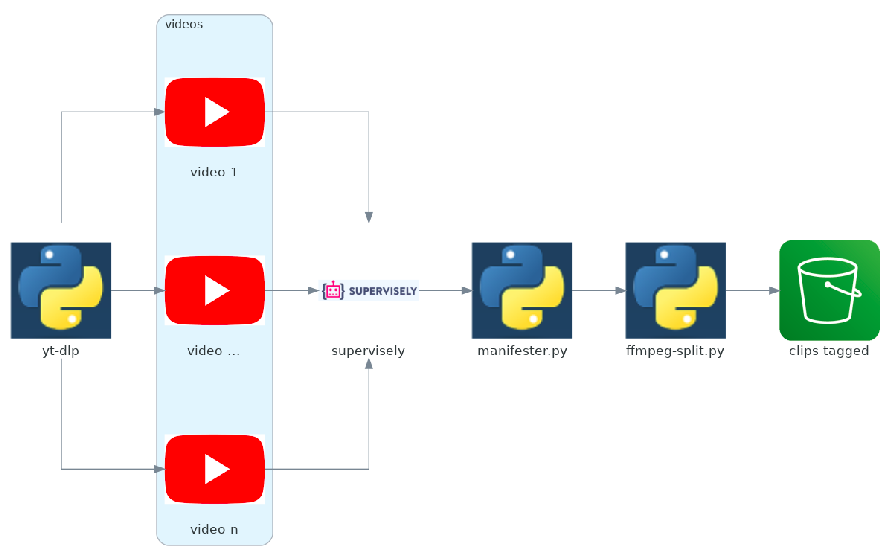
\includegraphics[width=\textwidth]{figs/data_extraction_process_.png}
\caption{Proceso de extración de datos}\label{data_extraction_process}
\end{figure}

Se descargan los videos utilizando \texttt{download.py}, y se procesan en \textit{Supervisely}. El output de \textit{Supervisely}, se transforma por medio de \texttt{manifester.py}, cuyo output se utiliza a su vez por \texttt{ffmpeg-split.py}, junto con los videos originales, para obtener los clips etiquetados, que se almacenan en un bucket de S3.

\subsection{Datos obtenidos}

En la tabla \ref{table_descriptive_stats} podemos ver los estadísticos descriptivos (media y desviación típica) del número de frames de todos los videos y duración (en segundos), desglosado por movimiento.

\begin{table}[htbp]
\centering
\caption{Estadísticos descriptivos de los frames y duración de los clips}
\label{table_descriptive_stats}
\begin{tabular}{l|lc|lc}
\toprule
{} & \multicolumn{2}{c|}{\textbf{Frames}} & \multicolumn{2}{c}{\textbf{Duración (s)}} \\
{} &    Media & Desviación típica &        Media & Desviación típica \\
\midrule
\textbf{thruster}          &  27.7396 &            4.5060 &       0.9419 &            0.1274 \\
\textbf{chest-to-bar}      &  21.0478 &            7.4233 &       0.7196 &            0.2569 \\
\textbf{double-unders}     &  14.5880 &            1.2740 &       0.4841 &            0.0439 \\
\textbf{ghd}               &  58.9732 &            5.5611 &       1.9654 &            0.1860 \\
\textbf{power clean}       &  67.3567 &           13.0092 &       2.2448 &            0.4337 \\
\textbf{deadlift}          &  24.1229 &            7.1950 &       0.8048 &            0.2395 \\
\textbf{shspu}             &  43.2100 &           15.1247 &       1.4412 &            0.5055 \\
\textbf{ohs}               &  31.9767 &            5.4303 &       1.0664 &            0.1799 \\
\textbf{bar-facing burpee} &  62.0233 &           10.0239 &       2.0688 &            0.3340 \\
\textbf{TOTAL}             &  39.0042 &           7.7275  &       1.3041 &            0.2563 \\
\bottomrule
\end{tabular}
\end{table}


Podemos observar que el movimiento más rápido (aquél con menor duración) es el \textit{double-under}, con $14.5580$ frames en media, y algo menos de medio segundo de duración ($0.4841$ segundos), mientras que el movimiento de mayor duración en media es el \textit{power clean}, con $67.36$ frames y $2.44$ segundos de media. Habría que tener en cuenta, que si bien los \textit{double-unders} son muy similares, el \textit{power clean} podría bajar de tiempo si se tomase una muestra de eventos diferente. Esto es debido a que en el evento escogido el peso con el que se realiza el movimiento es relativamente alto para este levantamiento.

Si comparamos con \href{https://www.crcv.ucf.edu/data/UCF101.php}{UCF101} por ejemplo, la longitud de los videos es menor en este dataset (en UCF101 la duración de los videos está alrededor de $7$ segundos, mientras que en \href{https://www.deepmind.com/open-source/kinetics}{Kinetics 600} está alrededor de $10$ segundos).


\section{Experimentación con deep learning}\label{deep_learning}

\subsection{Introducción}

En esta sección se explica el modelo seleccionado y el tratamiento aplicado a los datos, el proceso de entrenamiento del modelo y los resultados obtenidos.

Se ha decidido utilizar la implementación de \textit{MoViNets} basada en  \texttt{tensorflow}. Aunque existe más de una implementación del modelo actualmente (ver \href{https://paperswithcode.com/paper/movinets-mobile-video-networks-for-efficient}{\textit{Papers with code}}), los autores han decidido utilizar este framework para el desarrollo del modelo, y han publicado el modelo junto con \textit{checkpoints} del mismo en el siguiente \href{https://github.com/tensorflow/models/tree/master/official/projects/movinet}{repositorio de GitHub}, así como en \href{https://tfhub.dev/google/collections/movinet/1}{\textit{tensorflow hub}}.

\subsection{Preprocesado de los datos}

De cara a construir la pipeline para el entrenamiento del modelo, se ha utilizado la API de \href{https://www.tensorflow.org/api_docs/python/tf/data/Dataset}{\texttt{tf.data.Dataset}} ya que permite la ingesta de un conjunto potencialmente grande de datos, así como el procesamiento de los mismos de forma eficiente (ver \href{https://www.tensorflow.org/guide/data_performance}{\textit{Better performance with the tf.data API}}).

El primer paso para generar el nuevo dataset para el entrenamiento, consiste en trans-formar los videos en formato .mp4 a .tfrecords (ver \href{https://www.tensorflow.org/tutorials/load_data/tfrecord}{\textit{TFRecord and tf.train.Example}}), un forma-to para guardar una secuencia de ficheros en binario, basado en \href{https://developers.google.com/protocol-buffers/}{protocol-buffers} de Google específico para \texttt{Tensorflow}.

Para simplificar todo el proceso desde la lectura de los datos hasta el entrenamiento del modelo y posterior consumo del mismo (inferencia), se ha desarrollado una pequeña librería, disponible en PyPI: \href{https://pypi.org/project/movinets_helper/}{\texttt{movinets\_helper}}\footnote{Aunque aún está pendiente de documentar por completo y añadir los tests correspondientes, todo el entrenamiento y tratamiento de datos se ha hecho por medio de esta librería.}. El paso a paso en el preprocesamiento de los datos se puede ver en el siguiente \href{https://plaguss.github.io/movinets_helper/how-to-guides/#how-to-create-a-dataset}{enlace}.

Un punto relevante al transformar el formato de los datos es el tamaño. Los dataset en formato \href{https://www.tensorflow.org/api_docs/python/tf/data/TFRecordDataset}{\texttt{tf.data.TFRecordDataset}} no son eficientes en cuanto al espacio que ocupan, se pierde la ventaja de la compresión que ofrecen los formatos mp4 en video, o jpg en imágenes por ejemplo. El dataset pasa de ocupar alrededor de 400Mb en la resolución y formato original, a ocupar algo menos de 10Gb una vez almacenados como \textit{TFRecords}. Esto ocurre a pesar de comprimir los ficheros por medio de gzip, almacenar solo 10 frames de cada vídeo y almacenando la resolución necesaria para entrenar la versión a2 base de \textit{MoViNets}.

A la hora de leer el dataset (podemos seguir la \href{https://plaguss.github.io/movinets_helper/how-to-guides/#how-to-ingest-a-dataset}{guía} para este proceso), todos los videos se reescalan de acuerdo al modelo seleccionado (224x224p para el caso de a2 base), y se escalan los valores en RGB para que se encuentren en el rango $[0, 1]$.

Para homogeneizar los datos de entrada se ha decidido fijar al número de frames para todos los videos a 10 ($\bar{f}=10$)\footnote{Ver en el paper original el tratamiento del \textit{frame rate}. Aunque en el paper original utilizan 50 frames para los videos (Kinetics 600 tiene videos de 10 segundos, a una tasa de 24fps), en este caso no es posible en movimientos como los \textit{double-unders} ya que son mucho más cortos.}. Debido a que los vídeos en este conjunto de datos son más cortos que los utilizados en el caso de \textit{Kinetics 600}, se ha seleccionado el número de frames como $\bar{f} = \min_v f_{v}$, donde $f_v$ es el número de frames del vídeo $v$. El menor número de frames corresponde a uno de los vídeos de \textit{double-unders}. Para aquellos vídeos con un número de frames mayor que $\bar{f}$, se seleccionan $\bar{f}$ frames equiespaciados.

En la siguiente imagen \ref{frames} podemos ver el ejemplo de uno de los \textit{clips} que entran en la muestra de entrenamiento. Se trata de un \textit{power clean}, donde se pueden ver las distintas imágenes que componen el \textit{clip}.

\begin{figure}[H]
    %\centering
    \centerline{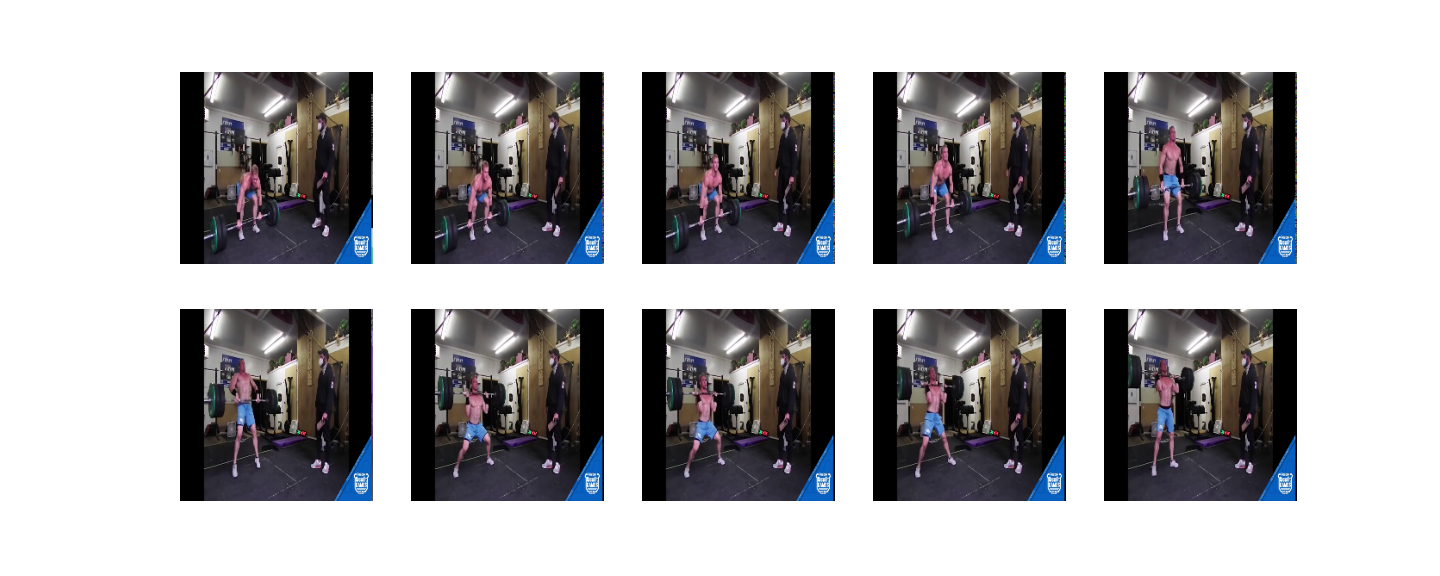
\includegraphics[width=1.25\linewidth]{figs/frames.png}}
\caption{Frames de una muestra de \textit{power clean} de la pipeline de entrenamiento}\label{frames}
\end{figure}

En el momento del entrenamiento, todos los videos están compuestos de 10 frames.

\subsection{Experimentos realizados y resultados}

El modelo se ha entrenado en \href{https://colab.research.google.com/?hl=es}{\textit{Google Colab}} con \textit{Tensorflow 2}. La versión y arquitectura seleccionada ha sido MoViNets A2 Base\footnote{No ha sido posible hacer fine-tuning del modelo Stream debido a un error en los modelos que han guardado los autores, ver \href{https://github.com/tensorflow/models/issues/10730}{issue 10730}.}, ya aunque sea necesario utilizar GPU para el fine-tuning, es el modelo más grande (y con mejor capacidad predictiva) que permite hacer inferencia con CPU en un tiempo razonable\footnote{En \href{https://blog.tensorflow.org/2022/04/video-classification-on-edge-devices.html}{este artículo} de \textit{Tensorflow} hacen referencia a aquellos modelos que pueden llegar a correr en tiempo real, considerando tiempo real como 20fps o superior.}.

Los hiperparámetros del modelo son los mismos utilizados en el paper original\footnote{Ver apartado \textit{B.1 More Details of the Architectures and Training} de \cite{MoViNets}}, con un tamaño de batch igual a 8\footnote{El tamaño del batch seleccionado es el mismo utilizado por los autores en el tutorial a modo de ejemplo sobre el dataset UCF101.}.

La muestra se divide en un $80\%$ (2164 clips) para training, y un $20\%$ (541 clips) para test, donde los ejemplos se distribuyen de manera balanceada (ver figura \ref{sample_sizes}).

\begin{figure}[H]
    \centering
		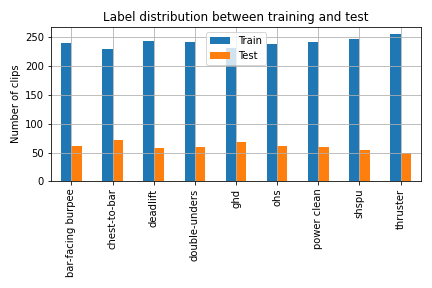
\includegraphics[width=\textwidth]{figs/sample_sizes.png}
\caption{Distribución de las etiquetas entre la muestra de entrenamiento y test}\label{sample_sizes}
\end{figure}

El modelo se ha entrenado durante 10 \textit{epochs}, evaluando top 1 y top 5 accuracy, obtenien-do un resultado de 0.9995 y 1 en entrenamiento y test respectivamente en top 1, como podemos observar en la siguiente imagen extraída de \textit{tensorboard.dev}:

\begin{figure}[H]
    \centering
		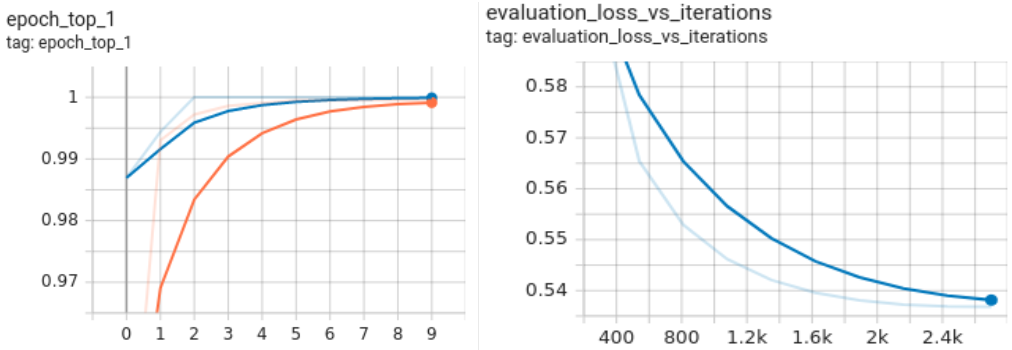
\includegraphics[width=\textwidth]{figs/tensorboard_training.png}
\caption{Top 1 categorial accuracy por epoch y loss por número de iteraciones}\label{training}
\end{figure}

El modelo base generaliza a un gran número de movimientos, incluyendo algunos movi-mientos similares\footnote{Por ejemplo, entre las  \href{https://raw.githubusercontent.com/tensorflow/models/f8af2291cced43fc9f1d9b41ddbf772ae7b0d7d2/official/projects/movinet/files/kinetics_600_labels.txt}{\textit{labels} de Kinetics 600} se encuentran \textit{squat}, \textit{clean and jerk} o \textit{snatch weight lifting}.} , lo que puede facilitar el aprendizaje de algunos de movimientos simila-res como puede ser en este caso el power clean o el thruster.

Por otro lado, los videos en este caso, aunque se han seleccionado de una muestra distinta de atletas, todos ellos son atletas de élite en su deporte, por lo que la ejecución de los movimientos son muy similares entre si, lo que facilita aprender a clasificar los mismos.

Los resultados del entrenamiento se pueden ver de forma interactiva en el siguiente enlace a \href{https://tensorboard.dev/experiment/UXyupsnMQ2S74vdul3vdbw/#scalars}{\textit{Tensorboard.dev}}. En vista de estos resultados, no ha sido necesario modificar nin-guno de los hiperparámetros propuestos por los autores del modelo.


\subsection{Evaluación de los resultados}

A la hora de evaluar los resultados, empezamos analizando el \textit{heatmap} de la matriz de confusión. Como se vio al analizar el accuracy en la muestra de test, todos los movimientos se clasifican bien (ver imagen \ref{training}).

\begin{figure}[H]
    \centering
		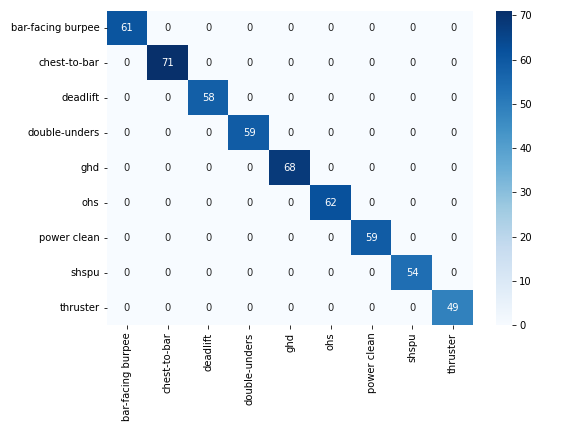
\includegraphics[width=\textwidth]{figs/heatmap_confusion.png}
\caption{Heatmap de la matriz de confusión para la muestra de test.}\label{app_3}
\end{figure}

Con vistas a proporcionar un análisis más robusto, en caso de que se decidiera extender el modelo a un mayor número de movimientos o muestras de distintos atletas, puede ser útil la información que proporciona el heatmap de la figura \ref{heatmap_correlations}. La construcción de este gráfico se hace de la siguiente forma:

Partiendo de las probabilidades asignadas a cada vídeo en el período de test, se fija para cada movimiento (cada \textit{label} correcta) y se calculan las correlaciones. Se selecciona la correlación (de Pearson) con el movimiento correctamente etiquetado, y se concatenan todos los vectores columna, de forma que obtenemos una matriz cuadrada. Estas correla-ciones ayudan a ver cuáles son los movimientos que más se "confunden" entre si. Dado que las probabilidades deben sumar 1, aquellos movimientos con una correlación negativa más cercana a 1, son aquellos en los que se puede observar una mayor intercambio de probabilidades respecto a la predicción correcta.

\begin{figure}[H]
    \centering
		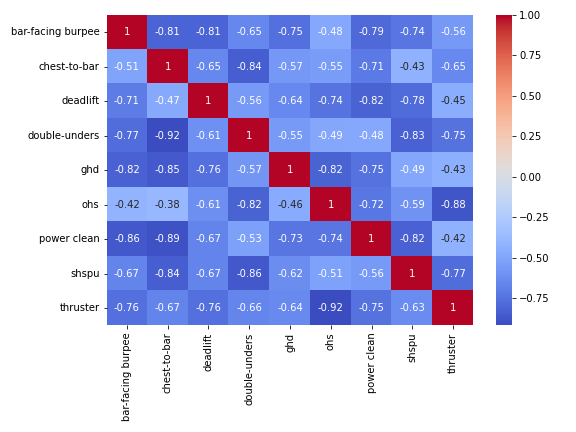
\includegraphics[width=\textwidth]{figs/heatmap_correlations.png}
\caption{Heatmap de correlación entre probabilidades. Para los clips clasificados como $j$, la celda $(i, j)$ representa la correlación entre las probabilidades de predecir el movimiento $i$ y el movimiento $j$.}\label{heatmap_correlations}
\end{figure}

Por ejemplo, si nos fijamos en la columna que corresponde a \textit{ohs}, vemos que el mayor coeficiente de correlación es de $-0.92$, con \textit{thruster}. Esto tiene sentido si se tiene en cuenta que en ambos movimientos, la barra parte de una sentadilla y acaba con la barra bloqueada por encima de la cabeza.

Por último, se puede ver en la siguiente tabla las probabilidades medias y desviación estándar obtenidas para cada movimiento correctamente etiquetado. Esto nos permite ver cuáles son los movimientos que se predicen con una mayor confianza, como en este caso los \textit{double-unders}, o los que menos, los \textit{ohs}. Las probabilidades que dan lugar a esta tabla se pueden ver en \ref{Probabilidades}.


\begin{table}[H]
\centering
\caption{Estadísticos principales }
\label{table_probabilities}
\begin{tabular}{lcc}
\toprule
{} &   Media &  Desviación típica \\
\midrule
double-unders     &  0.8921 &             0.0748 \\
ghd               &  0.8904 &             0.0533 \\
bar-facing burpee &  0.8876 &             0.0756 \\
thruster          &  0.8838 &             0.0590 \\
deadlift          &  0.8746 &             0.0796 \\
shspu             &  0.8731 &             0.0843 \\
chest-to-bar      &  0.8552 &             0.1282 \\
power clean       &  0.8443 &             0.0851 \\
ohs               &  0.8438 &             0.1163 \\
\bottomrule
\end{tabular}
\end{table}


\section{Cloud y despliegue de la aplicación}\label{despliegue}

\subsection{Introducción}

En el siguiente apartado se presenta la aplicación para clasificar movimientos de crossfit, la arquitectura elegida y su funcionamiento para un ejemplo en concreto.

Para la explotación del modelo se ha elegido desplegar una aplicación en AWS desarro-llada en Plotly Dash. Un usuario de la misma solo necesita subir un video en formato mp4 para recibir las predicciones del modelo para el movimiento. En los siguientes apartados se puede ver la arquitectura de la aplicación en la nube y los resultados obtenidos.

\subsection{Arquitectura cloud}

A continuación se puede ver en la figura \ref{cloud_diagram} el diagrama de la aplicación desplegada en AWS.

El punto de entrada para un usuario es la aplicación desplegada en \href{https://aws.amazon.com/es/ec2/}{\textit{EC2}}, cuyo código se puede ver en el repositorio \href{https://github.com/plaguss/movinets_dash_app}{\texttt{movinets\_dash\_app}}. La app está desarrollada en \href{https://plotly.com/dash/}{\textit{Dash}}, y ofrece la funcionalidad para subir un video en formato mp4 (y reproducirlo), obtener las probabilidades asociadas a cada movimiento, y mostrar ejemplos de los movimientos para los que se ha entrenado el modelo.

Se pueden distinguir dos bloques:
%
\begin{itemize}%
%
\item \textit{App pipeline}.
Por un lado tenemos la aplicación con la que interactúa el usuario.
Par-tiendo de un repositorio público en github que contiene el código del front end, por medio de \href{https://aws.amazon.com/es/codepipeline/}{AWS CodePipeline} y \href{https://aws.amazon.com/es/codedeploy/}{AWS CodeDeploy} se automatiza el despliegue de la misma en una instancia de \textit{EC2}, que viene desencadenado por medio de un \texttt{git push} a la rama master del repositorio.

\item \textit{Model predictions}.
Al subir un video, este se puede enviar a predecir (solo se reproduce en pantalla por defecto). El proceso en este caso contempla la interacción con el modelo por medio de una función \href{https://aws.amazon.com/es/lambda/}{\textit{AWS Lambda}}. Debido a las restricciones de tamaño de las funciones lambda, no es posible desplegar el código de la misma simplemente comprimiendo las dependencias, ya que tensorflow por si solo excede el límite mar-cado por AWS. El código de la lambda \href{https://github.com/plaguss/tfm-misc/tree/main/lambda_aws}{(ver aquí)} se debe empaquetar en Docker y subir la imagen a \href{https://aws.amazon.com/es/ecr/}{ECR}. La lambda se encarga por tanto de leer el video, cargar el modelo almacenado en S3, transformar el video al formato adecuado, y devolver las proba-bilidades asociadas al mismo por pantalla.

\end{itemize}


\begin{figure}[H]
    \centering
		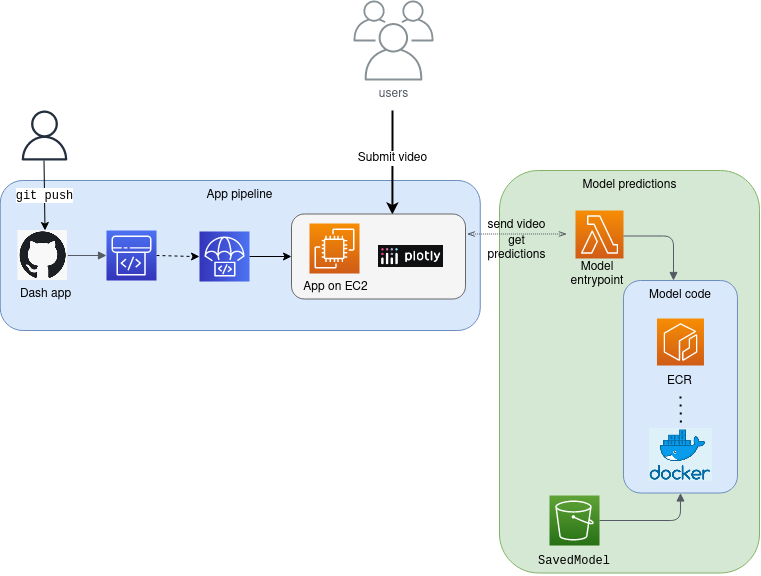
\includegraphics[width=\textwidth]{figs/cloud_diagram.png}
\caption{Diagrama Cloud}\label{cloud_diagram}


\end{figure}

\subsection{Resultado y funcionamiento}

A continuación se puede ver una serie de capturas de la app desplegada. La figura \ref{app_1} muestra la pantalla inicial de la app. La pestaña principal \textit{Clip prediction} permite cargar el vídeo arrastrando el archivo o buscándolo por su nombre. La pestaña secundaria \textit{Examples} permite ver ejemplos de los movimientos. 

\begin{figure}[H]
    \centering
		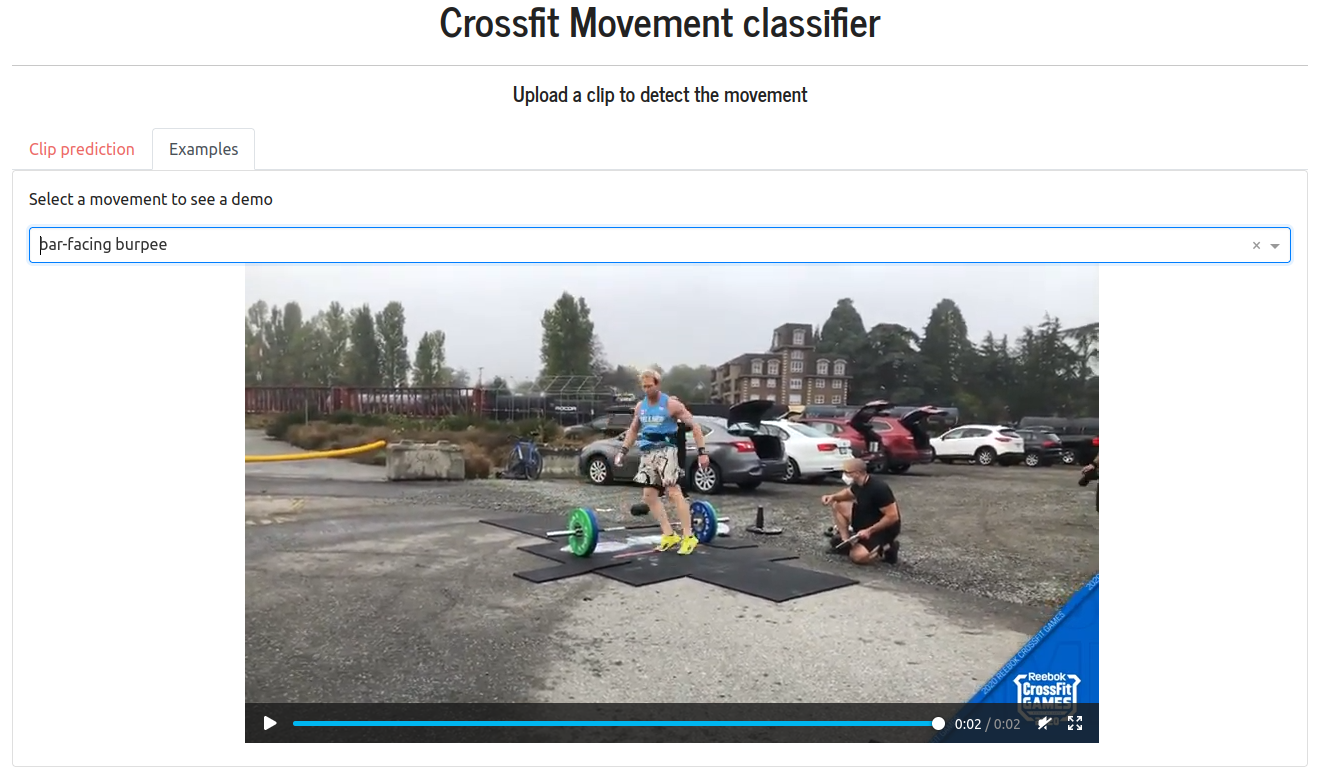
\includegraphics[width=\textwidth]{figs/bar-facing_burpee_example_app.png}
\caption{App: Estado inicial}\label{app_example}
\end{figure}


\begin{figure}[H]
    \centering
		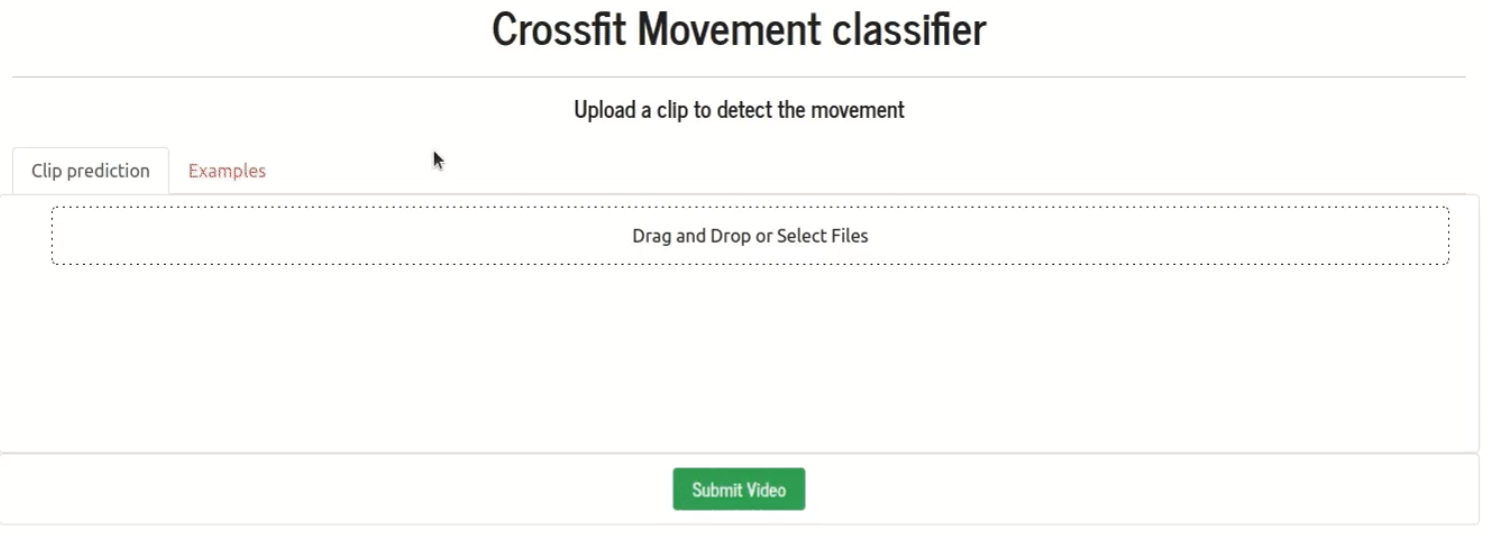
\includegraphics[width=\textwidth]{figs/app_1.png}
\caption{App: Estado inicial}\label{app_1}
\end{figure}

Una vez se ha subido un clip, este se reproduce de forma automática (imagen \ref{app_1} y \ref{app_2}). Para poder obtener las probabilidades asociadas al movimiento en cuestión habría que pulsar el botón \textit{Submit Video}, que envía el contenido a la función lambda.

\begin{figure}[H]
    \centering
		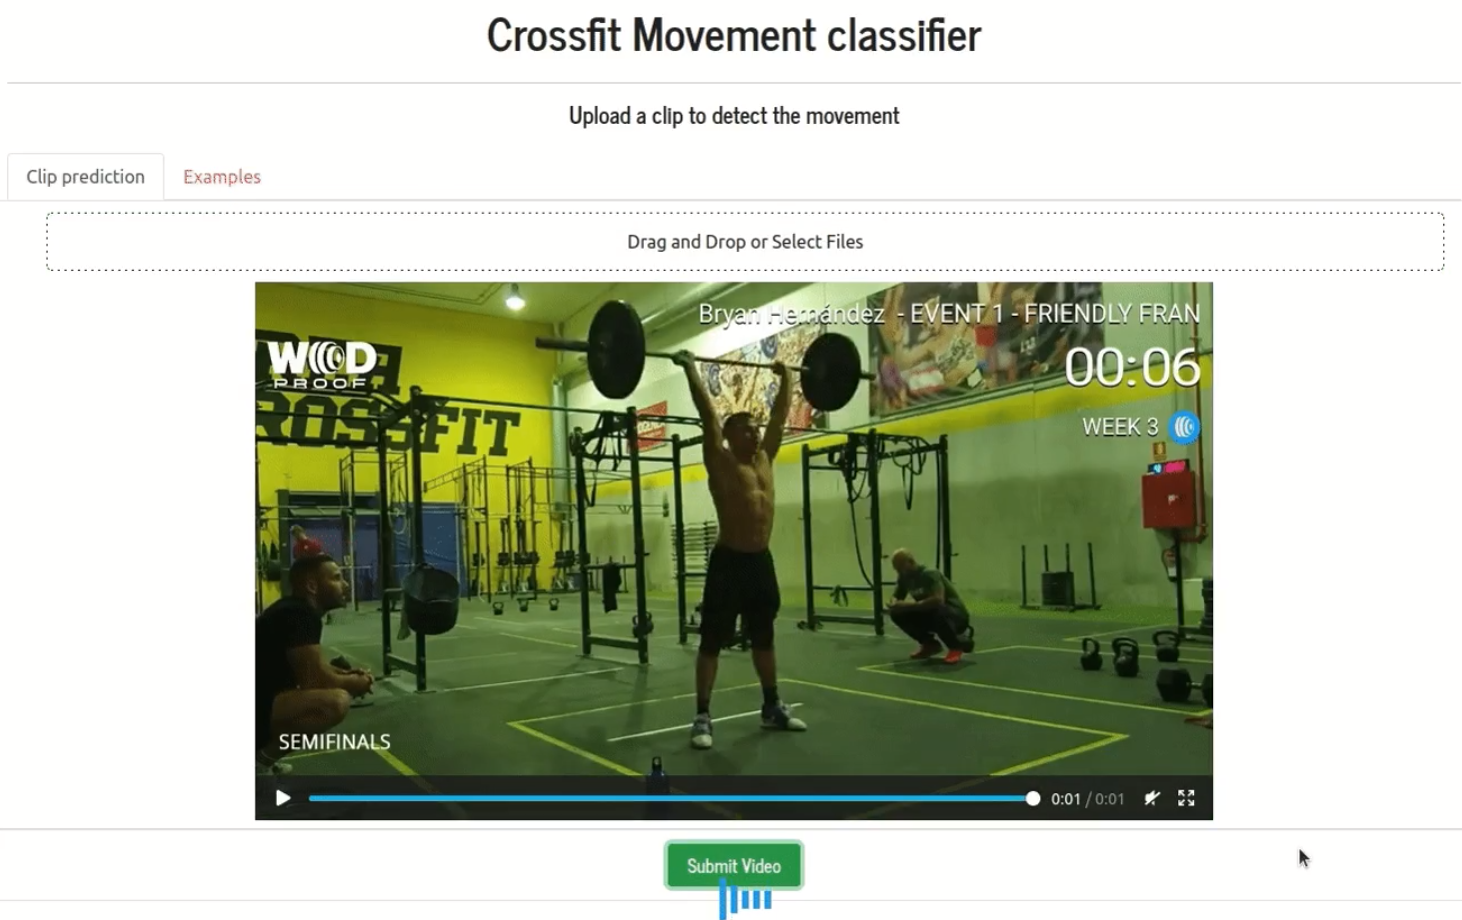
\includegraphics[width=\textwidth]{figs/app_2.png}
\caption{App: Video cargado}\label{app_2}
\end{figure}

Tras obtener la predicción del modelo, justo debajo aparece la tabla con los 5 movimientos más probables y la probabilidad asociada a cada uno de ellos, ordenados de mayor a menor, como muestra la figura \ref{app_3}.

\begin{figure}[H]
    \centering
		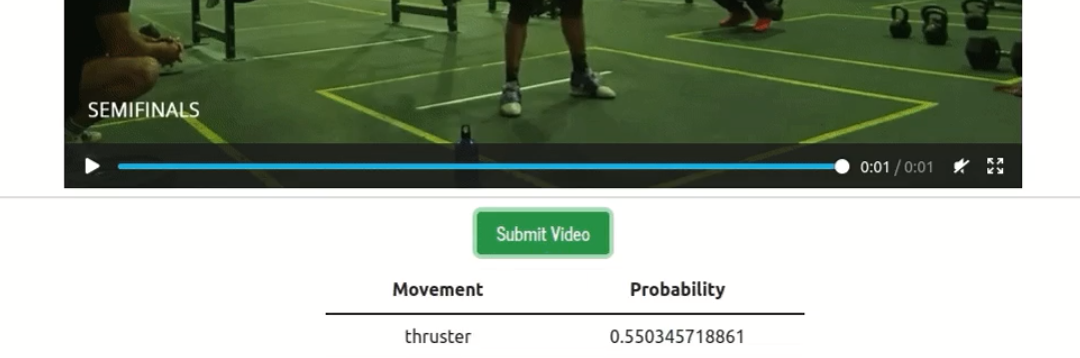
\includegraphics[width=\textwidth]{figs/app_3.png}
\caption{App: Extracto de tabla de predicciones}\label{app_3}
\end{figure}

Si bien los vídeos se han entrenado con un máximo de 10 frames, en este caso los vídeos se pasan al modelo sin hacer un muestreo de los mismos. Aunque solo se ha comprobado para unos pocos ejemplos de los vídeos completos, las probabilidades se ven afectadas, pero la ordenación de los mismos se mantiene.

El tiempo aproximado para obtener las predicciones asociadas a un clip es de alrededor de 14 segundos para un thruster, que es un movimiento relativamente corto (ver tabla \ref{table_descriptive_stats}), por lo que clasificar los movimientos es lento.

Como alternativas para ganar velocidad, se podría reducir el tamaño del modelo para mejorar la latencia de la CPU, limitando el número de posiciones decimales por ejemplo, un procedimiento conocido como \href{https://www.tensorflow.org/lite/performance/post_training_quantization}{\textit{post-training quantization}}. Los autores originales ofrecen versiones del mismo ya entrenadas para este caso \href{https://tfhub.dev/google/collections/movinet/1}{aquí}.

Existen otras alternativas. Se podría hacer un muestreo del vídeo de la misma forma que se hace durante la pipeline de entrenamiento (cabe recordar que durante el entrenamiento, el modelo solo utiliza 10 frames de cada vídeo), con lo que la información a procesar disminui-ría. Otra opción sería entrenar un modelo de menor complejidad, ya sea la versión a0 o a1, ya que el accuracy actual ya es excepcionalmente alto.



